\documentclass[../main.tex]
		
		\begin{document}
			\begin{description}
		\item[Task:] Introduce terminology related to graphs; understand different types of graphs; learn how to put together arguments involving graphs. \\
		An \underline{undirected graph} consists of:
		\begin{enumerate}
			\item A finite set of points $V$ called \underline{vertices}
			\item A finite set $E$ of \underline{edges} joining two distinct vertices of the graph.
		\end{enumerate}
		\item[Understand the meaning of an edge better:] Let $V$ be the set of vertices. Consider $P(V)$, the power set of $V$. Let $V_2 \subseteq P(V)$ consist of all subsets of $V$ containing exactly 2 points, \textbf{i.e.} $V_2 = \{A \in P(V) \mid \#(A)=2 \}$ \\
		Identify each element in $V_2$ with the edge joining the two points. In other words, if $\{a, b\} \in V_2$, then we can let $ab$ be the edge corresponding to $\{1, b\}$.
		\item[Examples:]
		\begin{enumerate}
			\item[]
			\item A traingle is an undirected graph. \\
			\begin{figure}[h!]
				\centering
				\begin{tikzpicture}
					\draw (0, 0) node[above]{A} -- (-1, -2);
					\draw (0, 0) -- (3, -2) node[right]{C};
					\draw  (-1, -2) node[left]{B} -- (3, -2);
				\end{tikzpicture}
			\end{figure}
			$V = \{A, B, C\}$ \\
			3 possible 2 element subsets of $V$:
			$\{A, B\} \rightarrow AB$ \\
			$\{A, C\} \rightarrow AC$ \\
			$\{B, C\} \rightarrow BC$ \\
			$E = \{AB, AC, BC\}$
			\item A pentagram is an example of an undirected graph. \\
			\begin{figure}[h!]
				\centering
				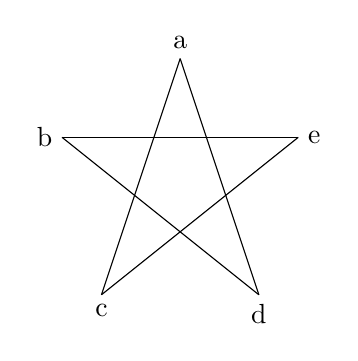
\begin{tikzpicture}
					\coordinate (A) at (0, 0);
					\coordinate (B) at (-1.5, -1);
					\coordinate (E) at (1.5, -1);
					\coordinate (C) at (-1, -3);
					\coordinate (D) at (1, -3);
					
					\draw (A) node[above]{a}--(C) node[below]{c};
					\draw (A)--(D) node[below]{d};
					\draw (C)--(E);
					\draw (D)--(B) node[left]{b};
					\draw (B)--(E) node[right]{e};
				\end{tikzpicture}
			\end{figure}
			$V = {a, b, c, d, e}$ \\
			$E = \{ac, ad, be, ce, bd\}$
		\end{enumerate}
		\item[Convention:] The set of vertices cannot be empty, \textbf{i.e.} $V \neq 0$.
		\item[Q:] If $V \neq \emptyset$, what is the simplest possible undirected graph?
		\item[A:] A graph consisting of a single point, \textbf{i.e.} with one vertex and two edges.
		\item[Definition:] A graph is called \underline{trivial} if it consists of one vertex and zero edges. Next, study how vertices and edges relate to each other.
		\item[Definition:] If $v$ is a vertex of some graph, if $e$ is an edge of that graph, and it $e = vv'$ for $v'$ another vertex, then the vertex $v$ is called \underline{incident} to the edge $e$ and the edge $e$ is called incident to the vertex $v$.
		\item[Example:] ~\\
		$b$ is incident to edges $be$ and $bd$ \\
		$be$ is incident to vertices $b$ and $e$
		\begin{figure}[h!]
			\centering
			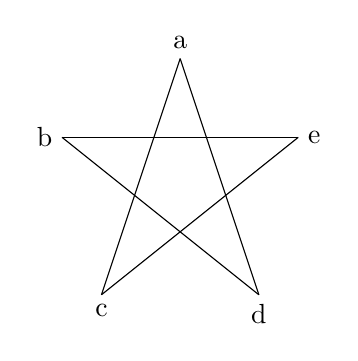
\begin{tikzpicture}
			\coordinate (A) at (0, 0);
			\coordinate (B) at (-1.5, -1);
			\coordinate (E) at (1.5, -1);
			\coordinate (C) at (-1, -3);
			\coordinate (D) at (1, -3);
			
			\draw (A) node[above]{a}--(C) node[below]{c};
			\draw (A)--(D) node[below]{d};
			\draw (C)--(E);
			\draw (D)--(B) node[left]{b};
			\draw (B)--(E) node[right]{e};
			\end{tikzpicture}
		\end{figure}
		\item[Definition:] Let $(V,E)$ be an undirected graph. Two vertices $A, B \in V \hspace{5mm} A \neq B$ are called \underline{adjacent} if $\exists$ edge $AB \in E$. \\
		We represent the incidence relations among the vertices $V$ and edges $E$ of an undirected graph via:
		\begin{enumerate}
			\item An incidence table
			\item An incidence matrix
		\end{enumerate}
		\item[Legend:] ~\\
		1 an incidence relation holds \\
		0 an incidene relation does not hold \\
		\item From the pentagram: \\
		$V = \{a, b, c, d, e\}$ \\
		$E = \{ac, ad, be, bd, ce\}$ \\
		\pagebreak
		\begin{figure}[h!]
			\centering
			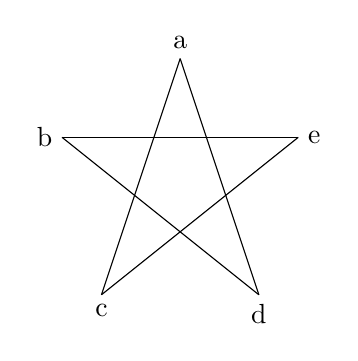
\begin{tikzpicture}
			\coordinate (A) at (0, 0);
			\coordinate (B) at (-1.5, -1);
			\coordinate (E) at (1.5, -1);
			\coordinate (C) at (-1, -3);
			\coordinate (D) at (1, -3);
			
			\draw (A) node[above]{a}--(C) node[below]{c};
			\draw (A)--(D) node[below]{d};
			\draw (C)--(E);
			\draw (D)--(B) node[left]{b};
			\draw (B)--(E) node[right]{e};
			\end{tikzpicture}
		\end{figure}
		\item The indidence table is:
		\begin{table}[h!]
			\centering
			\begin{tabular}{c|ccccc}
				& ac & ad & be & bd & ce \\ \cline{1-6}
				a & 1 & 1 & 0 & 0 & 0 \\
				b & 0 & 0 & 1 & 1 & 0 \\
				c & 1 & 0 & 0 & 0 & 1 \\
				d & 0 & 1 & 0 & 1 & 0 \\
				e & 0 & 0 & 1 & 0 & 1 \\
			\end{tabular}
		\end{table}
		\item Correspondingly, the incidence matrix is:
		\[ \left( \begin{array}{ccccc}
		1 & 1 & 0 & 0 & 0 \\
		0 & 0 & 1 & 1 & 0 \\
		1 & 0 & 0 & 0 & 1 \\
		0 & 1 & 0 & 1 & 0 \\
		0 & 0 & 1 & 0 & 1 \end{array} \right)\] 
		Note that for the incidence matrix to make sense, we need to know that vertices were considered in the order $\{a, b, c, d, e\}$ and edges in the order $\{ac, ad, be, bd, ce\}$. If we shuffle either set, the incidence matrix chances. \\
		With this in mind, we can now rigorously define the incidence matrix:
		\item[Definition:] Let $(V, E)$ be an undirected graph with $m$ vertices and $n$ edges. Let vertices be ordered as $v_1, v_2,\dots, v_m$, and let the edges be ordered $e_1, e_2, \dots, e_n$. The \underline{incidence matrix} for such a graph is given by $\left( \begin{array}{cccc}
			a_{11} & a_{12} & \dots & a_{1n} \\
			a_{21} & a_{22} & \dots & a_{2n} \\
			\vdots & \vdots & \ddots & \vdots \\
			a_{m1} & a_{m2} & \dots & a_{mn} \end{array} \right)$, where the entry $a_{ij}$ in row $i$ and column $j$ has the value 1 if the $i^{th}$ vertex is incident to the $j^{th}$ edge and has value 0 otherwise. \\
			Similarly, we can define the \underline{adjacency table} and the \underline{adjacency matrix} of a graph:
			\item[Definition:] Let $(V,E)$ be an undirected graph with $m$ vertices, and let these vertices be ordered as $v_1, v_2, \dots, v_m$. The \underline{adjacency matrix} for this graph is given by $\left( \begin{array}{cccc}
			b_{11} & b_{12} & \dots & b_{1m} \\
			b_{21} & b_{22} & \dots & b_{2m} \\
			\vdots & \vdots & \ddots & \vdots \\
			b_{m1} & b_{m2} & \dots & b_{mm} \end{array} \right)$ where $b_{ij}=1$ if $v_i$ and $v_j$ are adjacent to each other and $b_{ij}=0$ if $v_i$ and $v_j$ are not adjacent to each other.
			\item[Remark:] "Being adjacent to" is a symmetric relation on he set of vertices $V$, so the adjacency matrix is symmetric, \textbf{i.e.} $b_{ij}=b_{ji} \hspace{5mm} \forall i, j \hspace{5mm} 1 \leq i, j \leq m$. It is not reflexive so all the entries on the diagonal are zero.
	\end{description}
	
	\subsection{Complete graphs}
	\begin{description}
		\item[Definition:] A graph $(V, E)$ is called \underline{complete} if $\forall v, v' \in V$ s.t. $v \neq v'$, the edge $vv' \in E$. In other words, a complete grapg has the highest number of edges possible given its number of vertices.
		\item[Examples:] ~\\
		\begin{enumerate}
			\item The triangle is a complete graph.
			\item The pentagram is \underline{not} a complete graph.
		\end{enumerate}
		\item[Notation:] A complete graph with $n$ vertices is denoted by $K_n$.
		\item[Q:] How does the adjacency matrix of a complete graph look like?
		\item[A:] All entrices are 1 except on the diagonal, where they are all two.
		\item[Definition:] A graph $(V, E)$ is called \underline{bipartite} is $\exists$ subsets $V_1$ and $V_2$ s.t.
		\begin{enumerate}
			\item $V_1 \cup V_2 = V$
			\item $V_1 \cap V_2 = \emptyset$
			\item Every edge in $E$ is of the form $vw$ with $v \in V_1$ and $w \in V_2$.
		\end{enumerate}
		A bipartite graph is called a \underline{complete bipartite graph} if $\forall v \in V_1 \hspace{5mm} \forall w \in V_2 \hspace{5mm} \exists vw \in E$.
		\item[Notation:] A complete bipartite graph where the set $V_1$ has $p$ elements and the set $V_2$ has $q$ elements is denoted by $K_{p,q}$.
		\item[Example:] ~\\
		$V_1 = \{a, b\}$ \\
		$V_2 = \{c, d, e\}$ \\
		$V = \{a, b, c, d, e\}$ \\
		$E = \{ac, ad, ae, bc, bd, be\}$ \\
		\pagebreak
		\begin{figure}[h!]
			\centering
			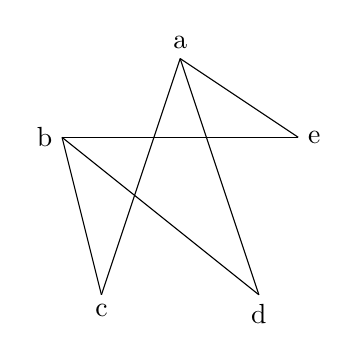
\begin{tikzpicture}
			\coordinate (A) at (0, 0);
			\coordinate (B) at (-1.5, -1);
			\coordinate (E) at (1.5, -1);
			\coordinate (C) at (-1, -3);
			\coordinate (D) at (1, -3);
			
			\draw (A) node[above]{a}--(C) node[below]{c};
			\draw (A)--(D) node[below]{d};
			\draw (A)--(E);
			\draw (B)--(C);
			\draw (D)--(B) node[left]{b};
			\draw (B)--(E) node[right]{e};
			\end{tikzpicture}
		\end{figure}
		is a complete bipartite graph.
		\item Next, relate graph to each other via functions with special properties.
	\end{description}
	

\end{document}